\documentclass[authoryear,review,12pt,number]{elsarticle}
\usepackage[utf8]{inputenc}
\usepackage[T1]{fontenc}
\usepackage[numbers]{natbib}
\usepackage{graphicx}
\usepackage{float}
\usepackage{rotating}
\usepackage{stfloats}
%\usepackage{lineno}
%\usepackage[linesnumbered,ruled,vlined]{algorithm2e}
\usepackage{tabulary}
\usepackage{graphicx}
\usepackage[none]{hyphenat}
%\usepackage[table]{xcolor} \sloppy
\usepackage[hyphens]{url}
\usepackage{hyperref}
\usepackage[toc]{glossaries}
\usepackage{amsmath}
\usepackage{multirow}
\usepackage{rotating}
\usepackage{adjustbox}
\usepackage{graphicx}% http://ctan.org/pkg/graphicx
\usepackage{booktabs}% http://ctan.org/pkg/booktabs
\usepackage{xparse}% http://ctan.org/pkg/xparse
\usepackage{booktabs}
\usepackage{array}
\usepackage[ddmmyyyy]{datetime}
\usepackage{listings}
\usepackage{color}
\usepackage{standalone}
\usepackage[final]{pdfpages}
\sloppy
\hypersetup{
    colorlinks=true,
    linkcolor=black,
    filecolor=magenta,      
    urlcolor=cyan,
    citecolor=blue,
}
\renewcommand{\dateseparator}{.}

\newcolumntype{R}[2]{%
    >{\adjustbox{angle=#1,lap=\width-(#2)}\bgroup}%
    l%
    <{\egroup}%
}
\newcommand*\rot{\multicolumn{1}{R{60}{1em}}}% no optional argument here,
% please!

\loadglsentries[main]{./glossary}
\makeglossaries
\begin{document}
%\begin{titlepage}
\begin{center}
{Author's Declaration}
\end{center}
I hereby certify that I am the sole author of this master thesis. 
Furthermore, I confirm that no sources have been used in the preparation of this thesis other
than those indicated in the thesis itself. The works of other people included in
my thesis, published or otherwise, are fully acknowledged in accordance with the
standard referencing practices. This thesis has not been submitted for another
degree or master to any other University or Institution.
\\
\\
Hiermit versichere
ich, dass ich die vorliegende Arbeit selbstst�ndig verfasst und keine anderen als die
angegebenen Quellen und Hilfsmittel benutzt habe. Alle Ausf�hrungen, die anderen
ver�ffentlichten oder nicht ver�ffentlichten Schriften w�rtlich oder
sinngem\"a\ss entnommen wurden, habe ich kenntlich gemacht. Die Arbeit hat in
gleicher oder \"ahnlicher Fassung noch keiner anderen Pr\"ufungsbeh\"orde vorgelegen.

\vfill
\begin{center}
\noindent
\begin{minipage}{0.5\textwidth}
\begin{flushleft}
\rule{5cm}{0.4pt}
Date/Datum 
\end{flushleft}
\end{minipage}%
\begin{minipage}{0.5\textwidth}
\begin{flushright} 
\rule{5cm}{0.4pt}
Signature/Unterschrift
\end{flushright}
\end{minipage}


\end{center}
\end{titlepage}
\begin{frontmatter}
%\linenumbers
\title{Combining machine learning and ontological data handling for multi-source
classification of nature conservation areas}
% Über den Titel muessen wir nochmal diskutieren. 

\author[TUB]{T. Niklas Moran\corref{cor1}}
\ead{niklasmoran@mailbox.tu-berlin.de}

\author[TUB]{Simon Nieland}
\author[TUB]{Birgit Kleinschmit}

\address[TUB]{Geoinformation in Environmental Planning Lab, Technische
Universit\"at Berlin, Stra\ss e des 17. Juni 145, 10623 Berlin, Germany}

\cortext[cor1]{Corresponding author at: Geoinformation in Environmental Planning
Lab, Technische Universit\"at Berlin, Stra\ss e des 17. Juni 145, 10623 Berlin,
Germany}

\begin{abstract}
Biodiversity monitoring using remote sensing (RS) is critical to meet 
requirements of existing laws such as the EU Habitats Directive and more 
importantly meet future challenges. The full potential of RS has yet to be 
harnessed as different nomenclatures and procedures hinder interoperability, 
comparison and provenance. Furthermore, manual field surveys are expensive 
and time-consuming. To meet these future challenges automated tools are needed 
to use RS data to produce comparable, empirical data outputs that lend 
themselves to data discovery and provenance. These issues are addressed by a 
novel semi-automatic ontology-based classification method that uses data mining 
algorithms and OWL ontologies that yields traceable, interoperable and 
observation-based classification outputs. The method is tested on EUNIS 
grasslands in Saarburg, Rheinland-Palatinate. The method is a first step in 
developing observation-based ontologies in the field of nature conservation. 
especially for data discovery, automatic image interpretation, data 
interoperability, workflow management and data publication.
\end{abstract}

\begin{keyword}
remote sensing, biotope classification, data mining, nature conservation, OWL, 
EUNIS, GEOBIA 
\end{keyword}
\end{frontmatter}
%\linenumbers
\section{Introduction}
Recognizing the importance of functioning ecosystems to reduce biodiversity 
loss, the European Union has implemented an environmental conservation 
framework to protect and conserve vital habitats in accordance with the 
Convention on Biological Diversity. An integral part of this framework is the 
EU Habitats Directive (Council Directive) 92/43/EEC [1992], which established 
the Natura 2000 network of habitats. The directive requires member states to 
conserve and monitor designated habitats and for a report to be submitted every 
six years. Environmental data to determine biodiversity status must be 
collected to comply with reporting requirements. Yet, comparing data used for 
these reports is difficult due to varying data collection methods and 
acquisition nomenclatures by the nature conservation authorities in each member 
state ~\citep{VandenBorre2011}. The main issue lies in the subjective nature of 
field surveys to identify habitats ~\citep{Cherrill1999, Cherrill1999a, 
Hearn2011, Nieland2015a}. Furthermore, habitat status is mostly generated in 
bottom-up approaches taking into account the national and regional 
interpretation guidelines ~\citep{VandenBorre2011, INSPIREdataspecs}. This 
subjective and time-consuming task of conducting field surveys could be 
partially replaced with an automated \gls{rs} method that uses \gls{geobia} to 
reduce subjectivity, costs and time.

Remote sensing offers opportunities to collect and automatically interpret 
large amounts of computer-readable data useful for nature conservation and 
biodiversity monitoring ~\citep{Corbane2015, VandenBorre2011, Mayer2011}. 
\gls{rs} image analysis implicitly incorporates the expertise of the person 
performing the analysis, reducing reproducibility as the analyst ultimately 
chooses class membership in non-crisp boundaries between classes. This can be 
divided into remote sensing knowledge (spectral signature, remote sensing 
indices, etc.) and field knowledge (feature properties, spatial relations, 
etc.) ~\citep{Andres2013a}, which is often neither completely nor explicitly 
defined as it is based on trial and error but influences the classification 
~\citep{Arvor2013}. To ensure accuracy and applicability of classification 
outputs for conservation, experts with detailed knowledge of the sites are 
needed to interpret the \gls{rs} data. The distance between the high-level 
semantics used by experts to describe domain concepts and the low-level 
information quantified from data is referred to as the ``semantic 
gap''~\citep{Smeulders00}.

Ontologies can help bridge the ``semantic gap'' and allow for better data 
transferability, knowledge and workflow management (provenance) and logical 
consistency ~\citep{Janowicz2012}. The standards-compliant format designed and 
adopted to express rich semantics and enable the ``Semantic Web'' is called the 
(\gls{owl})\footnote{\url{http://www.w3.org/TR/owl2-overview/}}. The format 
supports multiple syntaxes yet defines the \gls{rdf} (subject, predicate, 
object triplets) saved as \gls{xml} as a common exchange format. Moreover, 
through the use of reasoners (inference engines) that infer logical 
consequences over axioms and asserted facts and verify consistency, one can 
discover new knowledge ~\citep{Arvor2013, Andres2013a} \gls{rs} and field expert 
knowledge can be digitized in ontologies, thus allowing for a hierarchy of 
concepts for improved automatic image annotation and retrieval using concepts 
from both fields to produce more accurate results ~\citep{Srikanth2005}. 
~\cite{Janowicz2012} advocates for more observation-driven ontologies and for 
including machine learning, statistics and data mining to construct ontological 
primitives. While published research on using observation-based ontologies for 
biotope classifications is limited, the available research using ontologies in 
\gls{rs} research is briefly summarized below.

Ontologies modeled on the Land Cover Classification System and the General 
Habitat Category were integrated into tools used to monitor and protect areas 
in the EU ~\citep{Arvor2013}. The authors note that using the taxonomy of the 
different classification systems makes it possible to include expert knowledge 
in the process. ~\cite{Lucas2015} used pixel-based analysis and \gls{geobia} 
for greater classification accuracy which relies on a rule-base created by an 
expert. Other research includes classification of urban building types using a 
three-layered architecture ~\citep{diSciascio2013} and a semi-automated 
classification of urban building using the Random Forest classifier to 
determine variable importance of features from airborne laser scanner data 
~\citep{Belgiu2014}. Ontologies have also been paired with different algorithms 
to automatically acquire classification rules: a genetic programming algorithm 
~\citep{Forestier2012470} and the C4.5 data mining algorithm 
~\citep{Sheeren2006ML}. In biodiversity monitoring research, ontologies have 
been demonstrated to improve spatial data interoperability 
~\citep{Nieland2015a, Nieland2015b} and have been shown to aid in discovery of 
new relationships to consider for habitat management ~\citep{Perez-Luque2015}. 
The addition of fuzzy data types to \gls{owl} and the development of a fuzzy 
spatial reasoner holds great promise for the future of \gls{geobia} ontology 
research using remote sensing ~\citep{Belgiu2013, Bobillo2015}. More recently a 
multi-scale fuzzy spatial reasoner was developed which could have significant 
impact on this research ~\citep{Argyridis2015}.

Even though researchers recently developed a number of indicators using 
different sensors for habitat evaluation ~\citep{Nagendra2013}, classification 
procedures and rule-sets were not formalized to be computer readable and 
therefore suffer from similar transferablity and reproducibility problems as 
manual habitat mapping ~\citep{Arvor2013, Nieland2015a, Nieland2015b}. 
Therefore a formalized computer-readable ontology could help solve these 
problems and allow scientists to see how the classification was performed and 
be aware of possible incompatibilities before combining data 
~\citep{Janowicz2012}. Furthermore, there is no standardized set of indicators 
using \gls{rs} for trans-national habitat evaluation ~\citep{Lucas2015, 
VandenBorre2011}. Therefore, technical solutions to increase interoperability 
by thematically harmonizing environmental data and systematize data collection 
methods from remote sensing inputs in an automated workflow are needed. 

The \gls{eagle} is an expert group that seeks to harmonize \gls{lc}
and \gls{lu} nomenclatures using an object-oriented data model that 
eases translations between nomenclatures ~\citep{arnold2013eagle}. The many 
different nomenclatures used in Europe each have their own specific thematic 
conceptualization suited towards a specific scale and data collection method- 
reducing the ability to compare thematic maps. Since LU and LC are 
interconnected and influence one another, nomenclatures often incorporate both 
definitions into one class making separation difficult. To overcome this 
problem the \gls{eagle} data model describes landscapes in three main 
components: land cover (abiotic, vegetation, water) land use (agriculture, 
forestry, etc.) and characteristics (bio-physical, cultivation etc). The 
increased interoperability and transferability of \gls{rs} data and the 
semantic layer on top helps decision-makers to better assess and compare 
outcomes. 


In this paper we propose an automated system that can classify dry, mesic and 
wet grassland habitats according to the \gls{eunis} biotope classification 
schema using earth observation data, existing thematic maps (biotope, forestry, 
etc.), and expert knowledge formalized in an ontology by taking into account 
rules generated by data mining algorithms. The combination of data mining 
algorithms with ontology-based classification has, to our knowledge, not yet 
been done and is a first in remote sensing research. This method contributes to 
the goal of empirically-derived rule creation and enhances data 
interoperability and comparison as proposed ~\cite{Janowicz2012}. The main 
goals of this paper are:
\begin{itemize}
 \item to develop a \gls{rs} classification methodology using data mining 
approaches
     in combination with ontological formalism to generate highly interoperable,
     reproducible and exchangeable classification procedures and results,
 \item apply the methodology to indicators used to separate grassland habitats
     defined under \gls{eunis}
 \item and evaluate the developed approach by comparing it to a state-of-the art
     machine learning classifier \gls{et}
\footnote{\url{
http://scikit-learn.org/stable/modules/ensemble.html\#extremely-randomized-t
rees}}.
\end{itemize}

%%%%%%%%%%%%%%%%%%%%%%%%%%%%%%%%%%%%%%%%%%%%%%%%%%%%%%%%%%%%%%%%%%%%%%%%%%%%%%%%%
\section{Method}
%Hier muss eine kurze Einleitung fuer die Methode rein. Ich versuchs mal:
This section proposes an ontology-based classification approach which uses a
decision tree classifier for the semantic annotation procedure. It furthermore
describes the study area including available geo-data as well as the process of
semantic conceptualisation of classes in the nature conservation domain. To
evaluate the generated results the outcomes were compared to a highly randomised
tree classifier which is known to be suitable for this kind of classification
problem. %hier muss noch eine Quelle rein. Da gibts sicher ein benchmark von
% irgendwem
\subsection{Study area, data and classification nomenclature}
\label{sec:usecase_data}
%‚Testgebiet
%%%%%%%%%%%
Study area for this work is the administrative district of Saarburg. It extents
over an area of around 200km$^{2}$ and is
located in the south-west of the federal state of \gls{rlp}, Germany.
Luxembourg borders the area to the west and the federal state of Saarland to the
South. \gls{rlp} is influenced by western European atlantic climate and has an
economically and culturally important viticulture industry along the Mosel and Rhine rivers
(see figure \ref{fig:study_area}).
\begin{figure}
%Hier muss noch ein Nordpfeil und Massstab rein! 
    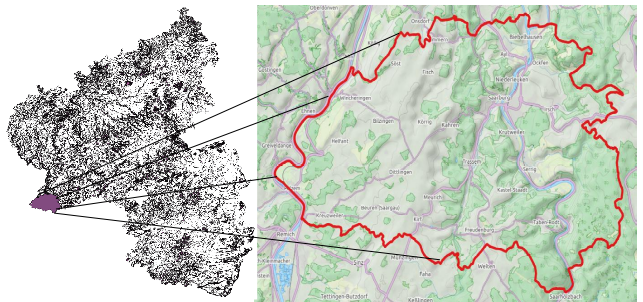
\includegraphics[width=\textwidth]{diagrams/study_area_closeup.png}
    \caption{The location of Saarburg (in purple) in relation to
    Rheinland-Palatinate. Map on right \copyright Thunderforest, Data\copyright
    OpenStreetMap contributors.}
\label{fig:study_area}
\end{figure}

% Nomenklatur %%%%%%%%%%%%%%%%
One of the main intentions of this work is to support the federal administration
of \gls{rlp} performing their regional biotope mapping as well as fulfilling its
European reporting obligations defined in the \gls{habdir}. Therefore we chose
the nomenclature of the \gls{eunis} to perform this research as it directly
satisfies the \gls{habdir} and has already been semantically transferred to the
local mapping nomenclatures. A consistent classification process could be realised by
describing \gls{eunis} classes with biophysical and anthropogenic indicators
which are supposed to be derivable with the help of the available data bases. To
achieve an accurate formalization of the regarded habitats, selected indicators
which are defined in \gls{eunis}, were adopted to meet the requirements of
remote sensing analysis.
Furthermore certain indicators of \gls{eagle}'s object-oriented data
model were used to describe land use, land cover and additional characteristics
(biophysical and anthropomorphic). The \gls{eagle} terms were adopted when possible to increase
interoperability and further re-use. Table ~\ref{tab:indicators_classes}
illustrates the regarded \gls{eunis} categories and subsequent descriptive
indicators.

\begin{table}
\centering
  \begin{tabular}{clcccccccc}
  \rot{\gls{eunis} class}&\rot{vegetation 
type} &\rot{wetness level} & 
  \rot{usage} & \rot{usage intensity} & \rot{immature
  soil} & \rot{hydromorphic} & \rot{species richness} \\ \hline
%\multirow{2}{*}{dry}
    E1   &  g/h & dry &g/m/- & low & 1 & 0 & 0/1/- \\ 
    E1.2 &  g/h & dry &g/m/- & low & 1 & 0 & 1\\
%\multirow{3}{*}{mesic} 
    E2   &  g/h & mesic &g/m/- & l/m/h/- & 0 & 0 & 0/1/-\\
    E2.1 &  g/h & mesic &g & medium/high & 0 & 0 & 0/1/- \\
    E2.6 &  g & mesic &g/m/- & high & 0 & 0 & 0 \\
%\multirow{2}{*}{wet}
    E3   &  g/h & wet & g/m/- & low/medium & 0 & 1 & 0/1/- \\
    E3.4  & g/h &  wet& g/m & medium & 0 & 1 & 0/1 \\
\end{tabular}
\caption{A `/ ' denotes OR and a '-' denotes 'none' and the first letter of 
each value is used to safe space. Vegetation type: \{graminaceous, 
herbaceous\}, usage: \{grazing, mowing\}, usage intensity: \{low, medium, 
high\}.}
\label{tab:indicators_classes}
\end{table}

%Referenzdaten
%%%%%%%%%%%%%%%%%
The thematic reference data consists of the federal biotope map (partially
updated 2015), agricultural data (updated every year) and a soil map which is
based on the ALKIS (Amtliches Liegenschaftskaster Informationssystem- Automated
Land Registration Map) (partially updated 2015).
In order to generate valid and consistent testing and training data for the
classification, these data were combined to create a comprehensive thematic
data basis for \gls{rlp} (see figure \ref{fig:pre-processing}). 
% The thematic maps include characteristics of \gls{lu},
% such as cultivation and management practice (grazing or mowing), biophysical
% characteristics (wetness, soil composition, morphology etc.) as well as land
% cover components (graminaceous vegetation, shrubs, trees, etc.).
To ensure the comparability of these base data sets they were characterised with
a common reference model of indicators, which have been developed on the basis
of the \gls{eagle} data model and the \gls{eunis} (see subsection
\ref{subsec:reference_data_and_semantic_characterisation}).
That means, all base data sets were conceptualised by using the developed
indicators (such as wetness, usage etc.) and can therefore be used as testing
and training data for certain categories which therefore serve as class labels
for the machine learning algorithm.

%Segmentierung
%%%%%%%%%%%%%%%%%%%%%
All described processes are based on a pre-segmented data set, generated using
\gls{geobia}. For this pre-segmentation step two types of data were taken into
account. Digital, multi-spectral (B, G, R, NIR) orthophotos (Year:2012-2013,
resolution 0.2m) and a \gls{dsm} (resolution 0.5m) which was generated by applying
automated stereo matching. These data therefore represent the basis for all
segmentation and classification procedures. 
The iterative object-based pre-classification was performed by
~\cite{Tintrup2015} in a multi-resolution
approach ~\citep{baatz2001ecognition}. A basic land cover extraction is performed by the
segmentation process which also follows the \gls{eagle} data model when
possible. This includes the main land cover classes trees, shrubs,
herbaceous/graminaceous vegetation, bare soil, heath, lichens and
mosses, reeds, artificial surfaces, water plants and forbs.

Furthermore, based on the available input data (\gls{dtm}, \gls{dem}
orthophotos), various zonal statistics could be calculated for the resulting
objects (see attachment BLABLA) (see figure \ref{fig:pre-processing}).


% Furthermore a \gls{dtm} and
% \gls{dem} was produced using \gls{lidar} ASCII point clouds acquired between
% 2003 and 2009 with a resolution of 0.2m. ? Fuer was wurde das benutzt?
% Vielleicht raus, oder?


Hence, the actual classification process is based on two RapidEye Scenes from 
2014 with 34 indices derived from the \gls{dtm}, \gls{dem} and orthophotos. 


%Graphik: cleanup wuerde ich nicht schreiben. Das sagt nichts aus. Vielleicht
% eher sowas wie ``assignment to common thematic/semantic reference model''.
% Statt segmented wuerde ich segmented data set schreiben. Und statt ``join'' wuerde
% ich ``calculation of zonal statistics'' schreiben. Mach vielleicht generell
% die Kaesten fuer die Datensaetze etwas groesser. Das sieht etwas gequetscht
% aus. Forestry kannst du raus machen. Das brauchen wir ja fuer grassland nicht.
% Mach doch die Raster input Daten auch noch mit in die Graphik! D.h. Dgm, RE,
\begin{figure} 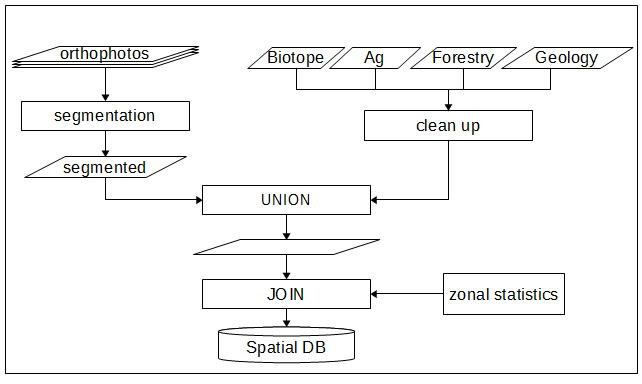
\includegraphics[width=1\textwidth]{diagrams/pre_processing.png}
    \caption{biotope, agriculture and soil maps were assigned to a
    common semantic reference model to generate comparability and then 
combined (union)
    and segmented objects, which were derived on the basis of digital
    orthophotos. To generate the base data for the classification, zonal
    statisitcs were calculated for all available raster data sets including
    sattelite (RapidEye) and airborne imagery and indices of the \gls{dem} and
    \gls{dtm}.
    \label{fig:pre-processing}}
\end{figure}


%%%%%%%%%%%%%%%%%%%%%%%%%%%%%%%%%%%%%%%%%%%%%%%%%%%%%%%%%%%%%%%%%%%%%%%%%%%%%%%%%%%%%%%
\subsection{Overview of the ontological classification process}
\label{subsec:method_overview}
Figure ~\ref{fig:full_workflow} gives an overview of the method using the
indicator \textit{wetness} as an example. The wetness level is essential to
differentiate dry, mesic and wet grassland habitats according to the second
level of the \gls{eunis} nomenclature (see table \ref{tab:indicators_classes}.
The developed system is comprised of (1) the preparation of reference
data, including a spatial union of the base data sets (pre-segmented,
pre-classified aerial photos and thematic maps (see
\ref{sec:usecase_data}) and the attachment of
subsequent semantic characteristics (see 
\ref{subsec:reference_data_and_semantic_characterisation}), (2)
the selection of training and validation data (see
\ref{subsec:Selection_of_training_validation_data}), the generation of
classification rules (see 
\ref{subsec:rule_generation}) using machine learning algorithms and
finally (4) the ontology-based classification process (see \ref{subsec:Onto_classification}). 

The software relies on a PostgreSQL database and various open source Python and 
Java libraries to interact with the database, convert files and execute a 
\textit{reasoner} over the created \gls{owl} ontology (see 
\ref{subsec:Onto_classification}). 
\begin{figure}
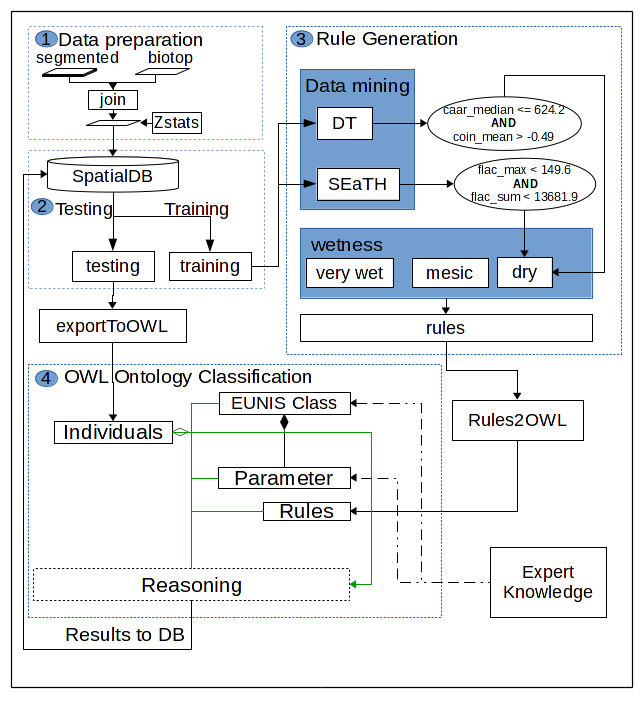
\includegraphics[width=1\linewidth]{diagrams/final_workflow_diagram.png}
\caption
    {
        1) The thematic maps (biotope, soil, etc.) are unioned together and
        spatial statistics are calculated for each combined polygon.
        2) Training and testing data are created and saved in the database.
        3) The rules are generated for e.g.\ the ``wetness'' indicator from
        training data.
        4) The rules are imported into the \gls{owl} ontology along with the 
testing
        data as individuals. The reasoner performs A-box reasoning to determine
        class membership.
    \label{fig:full_workflow}}
\end{figure}

% Furthermore, a reasoner can perform A-Box and T-Box reasoning over 
%the defined axioms.  Relationships between objects (subsumption, 
%disjointedness, etc). are  discovered and checked for consistency during T-box 
%reasoning. Using software,  such as Protege, users can see how the defined 
%axioms are related in the stored  knowledge base (\gls{owl}) and check for 
%logical consistency. If OWLIndividuals  (objects) are in the knowledge base 
%then A-Box reasoning can also be performed  finding if any of the individuals 
%fit into the defined classes. As \gls{eunis}  is an hierarchically structured 
%classification scheme testing that the  formalization follows the same 
%hierarchy is important. LC 

%%%%%%%%%%%%%%%%%%%%%%%%%%%%%%%%%%%%%%%%%%%%%%%%%%%%%%%%%%%%%%%%%%
\subsection{Semantic characterization}
\label{subsec:reference_data_and_semantic_characterisation} 
This step is crucial as the resulting segmentation output determines the 
quality of the later identification step as the data mining algorithms require 
characteristic biotopes to train on. 
Using \gls{eunis} class descriptions and
interpretation guidelines ~\citep{EUNISManual}, a set of indicators 
tailored to the available input data for our test area were created. Detailed
analysis of the \gls{eunis} nomenclature showed that some indicators do not lend themselves 
to easily be detected by \gls{rs} data. Therefore 
indicators were added to produce a meaningful formalization of the classes. The
formalization can be written to an \gls{owl} ontology, which is able to store 
complex logical connections (axioms) in an \gls{owl} file.

An \gls{owl} ontology is composed of classes, individuals and properties. 
Classes are sets of individuals and properties come in two forms: an object 
property defines a relationship between two individuals and a data property  
places a data type constraint on the individual ~\citep{OWL2}. 
We use environmental variables (e.g., wetness, soil maturity, vegetation type,
etc.) from the classification schemes and concepts from \gls{eagle} to preserve
interoperability by using this well-formalized vocabulary. All used indicators
for this research are shown in Table \ref{tab:indicators_classes}. An example of
a \gls{eunis} class, E2.22 ``Sub-Atlantic lowland hay meadows'' modelled with 
selected
remote sensing indicators is written in description logic (DL) below (see
equation ~\ref{eq:description_logic}).

\begin{tabular}[h]{p{0.8cm}l p{2cm}l}
    E2.22 &$\qquad$ {} $\equiv$ $\exists$has\_wetness \{``mesic''\} \\
      \ &$\qquad$ {} $\cap$ $\exists$has\_immature\_soil \{``false''\} \\
     &$\qquad$ {} $\cap$ $\exists$species\_richness \{``false''\} \\
\end{tabular}\label{eq:description_logic}\\


%Rule generation
%%%%%%%%%%%%%%%%%%%%%%%%%%%%%%%%%%%%%%%%%%%%%%%%%%%%%%%%%%%%
\subsection{Rule generation}
\label{subsec:rule_generation}

The \gls{dt} classifier was chosen as the base classifier for this methodology.
%Bitte such die Orginalquelle raus und zitier den dt classifier richtig.
It generates rules to separate indicator labels, such as dry, mesic
and wet which are then formalised in a OWL2 ontology to be able to use
ontology-based reasoning for classification purposes. To realise this task, the
\gls{dt} was parsed using a depth-first search algorithm. %
% bitte itzitieren!
Starting with the root node, the algorithm follows the left 
branch, visiting all children until it reaches the terminal leaf node. This 
branch lineage becomes the rule. The nodes of the \gls{dt} contain decision 
thresholds based on the supplied indices, the gini-coefficient and the values 
variable shows  
%?was bedeutet nochmal Value =??? Bitte dazu schreiben
% entropy!
the number of samples which were assigned to each class at that node (see 
figure 
\ref{fig:decisiontree}). All nodes visited before reaching the leaf node are 
chained with a logical ``AND'' together to create a rule. 

Based on the values variable the rule is
assigned to the class with the best accuracy, that means lowest rate in falsely
classified objects, %stimmt das????
 at that leaf node.
The process continues until all leaf nodes are visited. The rules are joined together by
logical ``OR"s and become a rule set for the indicator under investigation. An
example decision tree trained on the indicator class ‚\textit{wetness} is
depicted in figure \ref{fig:decisiontree}.%mach hier bitte ein durchgaengiges
% Beispiel! Einen Baum, eine zugehoerige Regel und eine formalisierung in OWL!
\begin{figure}
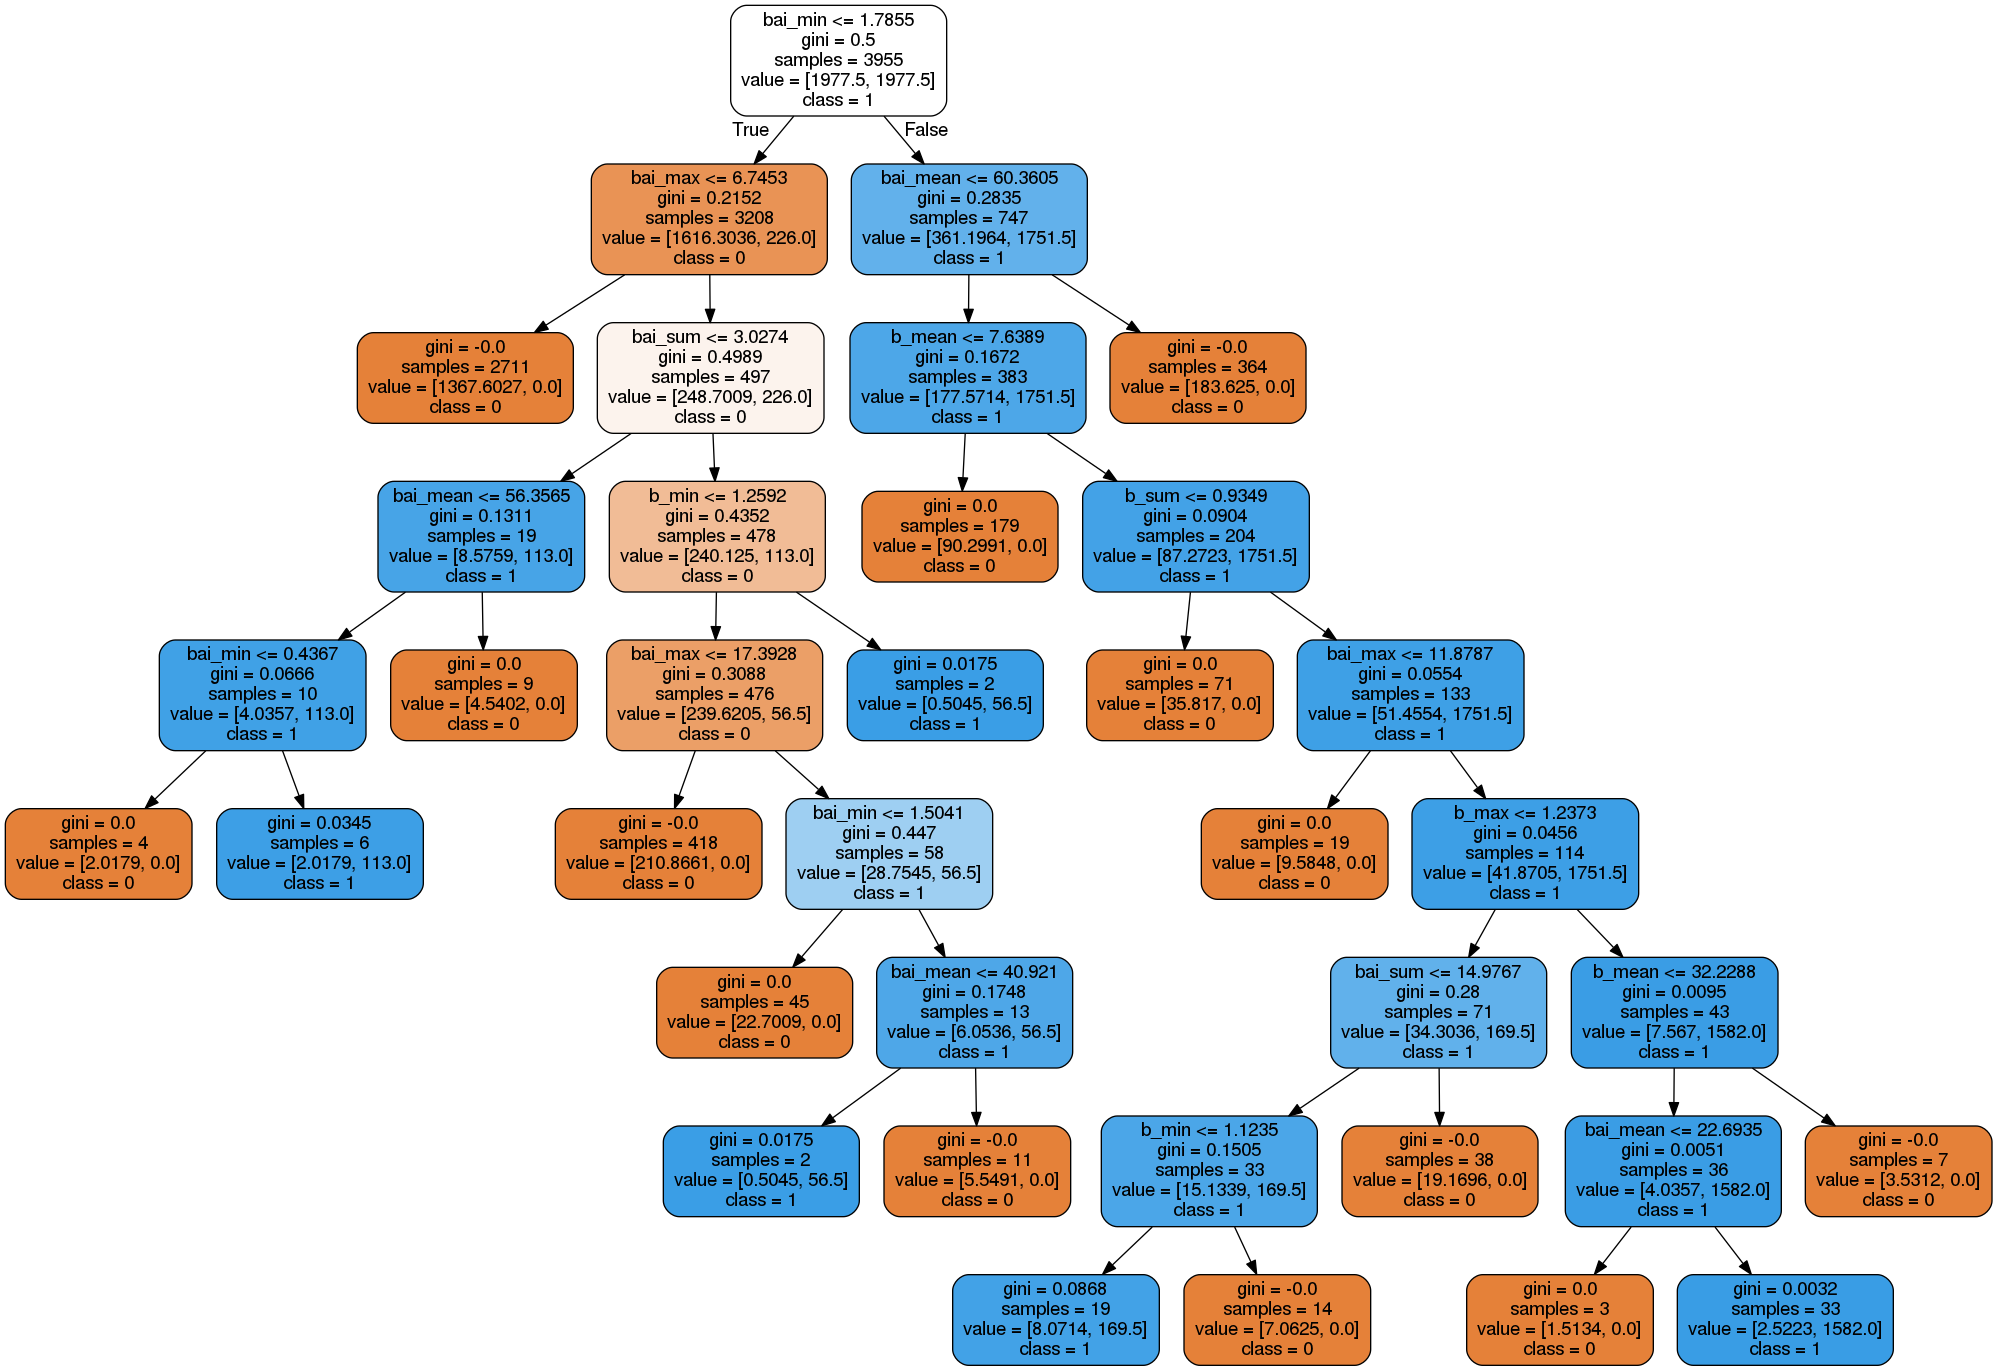
\includegraphics[width=\textwidth]{diagrams/natfo_immature_soil_dt.png}
    \caption{An example decision tree trained on immature soil 
indicator.\label{fig:decisiontree}}
\end{figure}

An example rule from the \gls{dt} is shown below. The subclass ``dry'' from
``wetness level'' has a rule that is generated by the decision tree algorithm as
seen in \ref{lst:dt_rule_snippet_csv} below. The first name is the
feature/statistic's name, followed by a threshold. For the \gls{dt}, the last
number is the node in the tree where the threshold comes from. This information
is currently not being used.
\lstset{language=XML,tabsize=2, label=lst:dt_rule_snippet_csv, caption=\lstname}
\begin{lstlisting}[frame=single]
    wief_max,>,1.092550,0
    tpi5_max,<=,-0.341000,420
    swi_median,<=,8.097600,421
    toin_max,<=,1536.561279,422
    pan4_glcm_std_135,<=,-7.890923,423
    b_std,<=,10.100981,424
\end{lstlisting}

\lstset{basicstyle=\footnotesize,language=XML,tabsize=2,
label=lst:dt_rule_snippet_owl , caption=\lstname, breaklines=true}
\begin{lstlisting}[frame=single,fontadjust]
            <DataSomeValuesFrom>
                <DataProperty IRI="#has_tpi5_max"/>
                <DatatypeRestriction>
                    <Datatype abbreviatedIRI="xsd:double"/>
                    <FacetRestriction facet="&xsd;maxInclusive">
                        <Literal datatypeIRI="&xsd;double">-0.341
                        </Literal>
                    </FacetRestriction>
                </DatatypeRestriction>
            </DataSomeValuesFrom>
            <DataSomeValuesFrom>
                <DataProperty IRI="#has_wief_max"/>
                <DatatypeRestriction>
                    <Datatype abbreviatedIRI="xsd:double"/>
                    <FacetRestriction facet="&xsd;minExclusive">
                        <Literal datatypeIRI="&xsd;double">1.09255
                        </Literal>
                    </FacetRestriction>
                </DatatypeRestriction>
            </DataSomeValuesFrom>
        </ObjectIntersectionOf>
    </ObjectUnionOf>
</EquivalentClasses>
\end{lstlisting}

\ref{lst:dt_rule_snippet_owl} shows how the first two lines of 
\ref{lst:dt_rule_snippet_csv} this rule look in an \gls{owl}/XML ontology. The 
rule has a collection of DataSomeValuesFrom within a nested datatype 
restriction 
corresponding to the rule threshold. A class can be defined by many rules 
containing multiple datatype properties that are chained together with logical 
AND (intersection) operators. The rules are then joined by a logical OR 
operator 
as can be seen in the outer ObjectUnionOf.


% %%%%%%%%%%%%%%%%%%%%%%%%%%%%%%%%%%%%%%%%%%%%%%%%%
\subsection{Ontology-based classification}
\label{subsec:Onto_classification}
After the algorithms produce rules for each indicator, these are then added as
facet restrictions to the \gls{owl} ontology. The polygons from the testing
table are loaded from the database as \gls{owl}Individuals into the same
ontology. Furthermore, a reasoner can perform A-Box and T-Box reasoning over the
defined axioms. In this procedure relationships between objects (subsumption,
disjointedness, etc) are discovered and checked for consistency during T-box
reasoning. Using software for ontology engineering and management, such as
Protege, users can see how the defined axioms are related in the stored
knowledge base (\gls{owl}) and check for logical consistency. If OWLIndividuals
(objects) are in the knowledge base then A-Box reasoning can also be performed
finding if any of the individuals fit into the defined classes. As \gls{eunis}
is an hierarchically structured classification scheme testing that the
formalization follows the same hierarchy is important.
In this work the reasoner FaCT++ was used to classify all polygons by applying
A-box reasoning over the rules. The classification results by the reasoner is
written to the database (see figure \label{fig:full_workflow}).

% %%%%%%%%%%%%%%%%%%%%%%%%%%%%%%%%%%%%%%%%%%%%%%%%%%%%%%%%%%%%%%%%%%%%%%%%
\subsection{Selection of training and validation data}
\label{subsec:Selection_of_training_validation_data}
The data was divided into 60\% for training and 40\% for validation. For the 
calibration and selection of suitable parameters for the classification 
algorithm the evolutionary search algorithm 
sklearn-deap\footnote{https://github.com/rsteca/sklearn-deap} was used based 
on the Distributed Evolutionary	Algorithms in Python (DEAP) 
~\citep{DEAP_JMLR2012}.
%Bitte hier % zitieren

%H.-G. Beyer and H.-P. Schwefel.   Evolution strategies:  A comprehensive
% introduction.
%Natural
%Computing
%, 1:3–52, 2002
%min_samples_leaf': 2, 'max_features': 'sqrt', 'criterion': 'entropy', 
%'min_samples_split': 4, 'max_depth': 10, 'class_weight': 'balanced'

The optimal parameters for the \gls{dt} were determined by using 10 evolutions, 
a population size of 50, tournament size of 3 and a gene mutation probability 
of 0.1 ~\citep{DEAP_JMLR2012} The parameters for the \gls{dt} that influence 
classification accuracy include: minimum samples leaf, minimum samples split, 
the max depth, the max features and the criterion ('entroy' or 'gini'). Two 
different fitted \gls{dt} classifiers were compared: Both were trained with a 
\gls{dt} and used the evolutionary search algorithm to find the best parameters 
to create the trees but one was fitted with all the features and the other with 
top 100 features as selected by \gls{et} classifier. Each \gls{dt} classifier 
undergoes a 5-fold cross validation to verify results and the \gls{dt} with the 
highest overall accuracy \gls{dt} was chosen.
\label{subsec:rulegen_data_mining}

%%%%%%%%%%%%%%%%%%%%%%%%%%%%%%%%%%%%%%%%%%%%%%%%%%%%%%%%%%%%%%%%%%%%%%%%%%
\subsection{Validation} 
\label{subsec:Validation}
For the training and testing of the described algorithm, only polygons greater
than 200m$^{2}$ were selected. Furthermore they had to be identified as
herbaceous or graminaceous plants according to the pre-segmentation and the 
the 90 percentile of the \gls{ndsm} had to be less than 1 meter. Therefore the
training and testing data includes polygons of grasslands between trees in
orchards and grasslands in agricultural production. Finally, to evaluate the
quality of the results in respect to well-established, popular classification
approaches the outcomes were compared to an \gls{et} reference classification
(see
\ref{tab:accuracy_indicators}
We use precision\footnote{\url{
http://scikit-learn.org/stable/modules/generated/sklearn.metrics.precision_score
.html\#sklearn.metrics.precision\_score}} (positive predicative value), 
recall\footnote{\url{
http://scikit-learn.org/stable/modules/generated/sklearn.metrics.recall_score.ht
ml\#sklearn.metrics.recall\_score}} (sensitivity, true positive rate), 
value) and 
f-score\footnote{\url{
http://scikit-learn.org/stable/modules/generated/sklearn.metrics.f1_score.html\#
s
klearn.metrics.f1\_score}} to determine the accuracy of classification results. 
The precision score (\ref{eq:precision}) is a reflection of how many of the 
objects that were classified were true positives. Recall \ref{eq:recall} shows 
the classifier's ability to find all relevant objects (positive samples). The 
f-score is the harmonic mean of the precision and recall.
\begin{equation}\label{eq:precision}
%\begin{align*}
    \frac{\text{true positives}}{\text{true positives + false positives}}
%\end{align*}
\end{equation}

\begin{equation}\label{eq:recall}
%\begin{align*}
    \frac{\text{true positives}}{\text{true positives + false negatives}}
%\end{align*}
\end{equation}
\begin{equation}\label{eq:fscore}
%\begin{align*}
    2 * \frac{\text{precision * recall}}{\text{precision + recall}}
%\end{align*}
\end{equation}
First the rules are generated for each indicator and the metrics in 
\ref{eq:precision}, \ref{eq:recall} and \ref{eq:fscore} are saved for accuracy 
analysis and for later scrutiny. The results for each indicator is saved in the 
database. Objects that meet the rule as defined in \ref{tab:indicators_classes} 
are assigned to that class. The classified result is then compared to the 
actual class label to determine the quality of the results.


%%%%%%%%%%%%%%%%%%%%%%%%%%%%%%%%%%%%%%%%%%%%%%%%%%%%%%%%%%%%%%%%%%%%%%%%%%%%%%%%
%Results
%%%%%%%%%%%%%%%%%%%%%%%%%%%%%%%%%%%%%%%%%%%%%%%%%%%%%%%%%%%%%%%%%%%%%%%%%%%%%%%%
\section{Results}
%%% MAY %%% 

\begin{tabular}{c | c c c c}
Class & Precision & Recall & F-score & Support\\
\hline
\hline\\
dry & 0.0 & 0.0 & 0.0 & 20\\
mesic & 0.99 & 0.99 & 0.99 & 2816\\
avg & 0.99 & 0.99 & 0.99 & 2836\\
\end{tabular}

%%% MNZ %%%

\begin{tabular}{c | c c c c}
Class & Precision & Recall & F-score & Support\\
\hline
\hline\\
dry & 0.0 & 0.0 & 0.0 & 5\\
mesic & 1.0 & 0.98 & 0.99 & 3521\\
wet & 0.0 & 0.0 & 0.0 & 4\\
avg & 0.99 & 0.98 & 0.99 & 3530\\
\end{tabular}
%% MAY %%%
\begin{table}
    \centering
    %\rowcolors{2}{lightgray}{white}
    \begin{tabular}{l l l l c c c }
    Indicator & Features & Class & Precision & Recall & F-score & 
    Support\\
    \hline
    \multirow{6}{*}{\rotatebox[origin=c]{90}{acidity}}
    & \multirow{3}{*}{\rotatebox[origin=c]{90}{all}} 
    & alkaline & 0.15 & 1.0 & 0.26 & 33\\
    & & null & 0.0 & 0.0 & 0.0 & 189\\
    & & avg & 0.02 & 0.15 & 0.04 & 222\\
    \cline{2-7}
    & \multirow{3}{*}{\rotatebox[origin=c]{90}{100}} 
    & alkaline & 0.02 & 1.0 & 0.03 & 60\\
    & & null & 0.0 & 0.0 & 0.0 & 3424\\
    & & avg & 0.0 & 0.02 & 0.0 & 3484\\
    \cline{2-7}
    \multirow{6}{*}{\rotatebox[origin=c]{90}{wetness}}
    & \multirow{3}{*}{\rotatebox[origin=c]{90}{all}}
    & dry & 0.0 & 0.0 & 0.0 & 20\\
    & & mesic & 0.99 & 0.99 & 0.99 & 2816\\
    & & avg & 0.99 & 0.99 & 0.99 & 2836\\
    \cline{2-7}
    & \multirow{3}{*}{\rotatebox[origin=c]{90}{100}}
    & dry & 0.0 & 0.05 & 0.0 & 59\\
    & & mesic & 0.88 & 0.12 & 0.2 & 3425\\
    & & avg & 0.86 & 0.11 & 0.2 & 3484\\
    \end{tabular}
    \caption{Overall classification accuracy of 
indicators\label{tab:accuracy_indicators}}
\end{table}
The poor performance of the wetness indicator negatively effects classification 
of the
biotopes. Luckily, the immature soil and hydromorphic indicators when combined
are disjoint (see \ref{tab:indicators_classes})
\subsection{EUNIS Level 2 Classification}
\label{subsec:level2_classification}
The \gls{dt} classifier has 4115 false
positives (19654 classified vs. 15539 actual) 
\begin{table}
\centering
\begin{tabular}{c c c c c}
Class & Precision & Recall & F-score & Support\\
\hline
E1 & 0.5 & 0.01 & 0.02 & 122\\
E2 & 0.79 & 0.58 & 0.67 & 15539\\
E3 & 0.7 & 0.11 & 0.2 & 61\\
unclass & 0.0 & 0.0 & 0.0 & 5376\\
avg & 0.59 & 0.43 & 0.49 & 21098\\
\end{tabular}
\caption{Classification accuracy of grasslands using the \gls{dt} 
classifier\label{fig:dt_lvl2_classification}}
\end{table}
% gibt es ueberhaupt I1 noch im Datensatz?!
The largest number of polygons in the testing data not belonging to \gls{eunis}
grasslands belong to I1 which are described as ``Arable land and
market gardens''. The class includes meadow/pastureland under management and
recently fallowed land under I1.5. 

The dominance of mesic grasslands in Saarburg is clearly reflected in
the results. In the testing data of the 21098 objects, 15539 objects - 74\% -
are mesic grasslands. Less than 1\% of objects are in E1 (122) and E3 (61). 
\begin{table}
\centering
\begin{tabular}{c c c c c}
Class & Precision & Recall & F-score & Support\\
\hline
E1 & 0.03 & 0.68 & 0.05 & 122\\
E2 & 0.68 & 0.01 & 0.02 & 15539\\
E3 & 0.02 & 0.38 & 0.04 & 61\\
unclass & 0.0 & 0.0 & 0.0 & 5376\\
avg & 0.5 & 0.01 & 0.01 & 21098\\
\end{tabular}
\caption{Classification accuracy of grasslands using the \gls{seath}
algorithm\label{fig:seath_lvl2_classification}}
\end{table}

%%%%

\subsection{EUNIS Level 3 classificaton}
\begin{table}
\centering
\begin{tabular}{c c c c c}
Class & Precision & Recall & F-score & Support\\
\hline
E1.2 & 0.5 & 0.01 & 0.02 & 122\\
E2.1 & 0.63 & 0.69 & 0.66 & 11509\\
E2.6 & 0.17 & 0.04 & 0.07 & 4335\\
E3.4 & 1.0 & 0.03 & 0.06 & 64\\
avg & 0.37 & 0.37 & 0.36 & 21788\\
\end{tabular}
\caption{Classification accuracy for \gls{eunis} level 3 using \gls{dt}}
\end{table}
\begin{table}
\centering
\begin{tabular}{c c c c c}
Class & Precision & Recall & F-score & Support\\
\hline
E1.2 & 1.0 & 0.01 & 0.02 & 122\\
E2.1 & 0.0 & 0.0 & 0.0 & 11105\\
E2.6 & 0.5 & 0.0 & 0.0 & 4240\\
E3.4 & 0.02 & 0.3 & 0.04 & 61\\
unclass & 0.0 & 0.0 & 0.0 & 5374\\
avg & 0.11 & 0.0 & 0.0 & 21098\\
\end{tabular}
\caption{Classification accuracy for \gls{eunis} level 3 using SEaTH}
\end{table}
At level three fewer objects are found and classified. Our indicators are not 
capable of detecting the differences at this level. For instance in dry 
grasslands there is only one object in E1.71, all the rest of the dry 
grasslands are in E1.262.

%Discussion
%%%%%%%%%%%%%%%%%%%%%%%%%%%%%%%%%%%%%%%%%%%%%%%%%%%%%%%%%%%%%%%%%%%%%%%%%
\section{Discussion}
As a base classifier for the proposed methodology the \gls{dt} was chosen.
Benefits of this machine learning algorithm are on the one hand the traceability
and understandability of the resulting rules, on the other hand \gls{dt} has
been utilised successfully for several related research questions 
~\citep{Franke2012125, Otukei2010S27}.


As can been seen in table \ref{tab:accuracy_indicators}, the immature soil and
hydromorphic indicators performed well. The poor performance of the wetness
indicator in particular is surprising as the data mining algorithms had 
access to many different wetness indicators and morphological data. Since 
classifying \gls{eunis} level 2 grasslands requires information on wetness, 
the classification suffers. The performance of usage and usage intensity is 
most likely due to a lack of time series data. In regards to algorithmic 
performance, SEaTH performed poorly overall and the results show that the 
\gls{dt} classifier achieves comparable results to the \gls{et} classifier 
for the indicators chosen. 

The very few dry grasslands in the Saarburg region hurt the classifier's 
ability to learn from the data. Only one dry grassland classified as such fits 
the rule's definition of a dry grassland. The reasons for this could be due the 
differences in data quality between the biotope map and the agriculture map. 
It could also be a conceptualization problem with the translation from the 
\gls{rlp} classification to \gls{eunis}.

Visually inspecting the data revealed that polygons were in fact grasslands, 
agricultural land or meadows. Most belonged the class I1 - ``Arable land and 
market gardens'' and the \gls{eunis} biotope classification guide specifically 
states that turf and sports fields are excluded. Since I1 is ``species poor'' 
adding ``species richness'' to the E2 rule reduced the number of polygons 
classified as I1 but also reduced the total number of E2 classes as well. Thus, 
adding species richness was not helpful. The height restriction and the class 
name ``herbaceous plants'' from the segmentation properly excluded trees, 
artificial buildings, etc. The larger size of the thematic map's polygons means 
that a polygon of grasslands in between an orchard will still be assigned the 
orchard's label and \gls{eunis} indicators. Early on the issue with orchards 
was identified as a troubling area for segmentation and this has not yet been 
resolved. A multi-scale approach will probably be needed to solve this problem. 

The selection of grasslands greater than 200m$^{2}$ in size might have also led 
to errors as max and min values in the \gls{dsm} had a large range. The 
pre-segmentation class herbaceous plants could be too lenient as shrubs were 
found in polygons labeled as herbaceous. In addition other indicators are 
needed to more accurately differentiate between grasslands.

Lastly, properly exploiting a dimension reduction strategy using principal 
component analysis or some other method could possibly improve the data mining 
algorithms classification accuracy. The addition of time series data for 
intensity and soil maps would greatly help classification accuracy.
\section{Conclusion}
The results demonstrate that the method provides additional value when compared 
with a normal classification approach and that with proper conceptualization, 
reference data and dimension reduction could achieve results comparable to an 
\gls{et} classifier. Furthermore, we tested the method on formalized 
\gls{eunis} grasslands and showed that it could be used to refine the 
indicators and revisit the conceptualization. 

Further investigation of the segmented polygons and a test area with a more
uniform distribution of biotope classes is needed. Accurate reference data is
needed to diagnose why the wetness indicator performed so poorly. Other 
algorithms should be applied for comparison.

We demonstrated that an ontological-based semi-automated classification system
produces interoperable and exchangeable classification outputs
and results and is not constrained by data mining
algorithms or software. Furthermore, such tools can be applied to different 
domains and, for biodiversity monitoring, help decision-makers make informed 
decision by being able to compare outputs.
\section{Acknowledgments}
We would like to thank \gls{rlp} AgroScience GmbH for processing the data and 
the \gls{rlp}'s Environment Ministry for funding the \gls{natflo} project. This 
work was conducted using the Prot\'eg\'e resource, which is supported by grant 
GM10331601 from the National Institute of General Medical Sciences of the 
United States National Institutes of Health.
\section{Appendix}
The \gls{owl} ontology with rules generated by the \gls{dt} algorithm used in 
this study is located at: 
\url{http://www.user.tu-berlin.de/niklasmoran/grassland_dt.owl} and the SEaTH 
\gls{owl} file is located: 
\url{http://www.user.tu-berlin.de/niklasmoran/grassland_seath.owl}
\bibliographystyle{model2-names}
\section{References}
\bibliography{references}
%\printglossary
\section{Appendix}
\begin{center}
\begin{tabular}{ll}
\label{tab:indices}
dtm/dem & orthophotos\\
aspect & red\\
catchment area & blue\\
convergence index & green\\
curvature classification & bare area index\\
Double Difference Vegetation Index & Normalized Difference Vegetation Index\\
Diurnal Anisotropic Heating & Normalized Difference Wetness Index\\
DIFI & Near Infrared\\
flow accumulaction & Panchromatic\\
Morphometric Protection Index & Red edge\\
MRRT & RapidEye(nir, red edge, r,g,b\\
Multiresolution Index of Valley Bottom Flattness & ×\\
Profile Curvature & ×\\
Slope & ×\\
SAGA Wetness Index & ×\\
Total Insolation & ×\\
Topographic Position Index & ×\\
Terrain Ruggedness Index & ×\\
Wind Effect & ×\\
Normalized Digital Surface Model & ×\\
× & ×\\
× & ×\\
× & ×\\
× & ×\\
× & ×\\
× & ×\\
× & ×\\
× & ×\\
× & ×\\
× & ×\\
× & ×\\
× & ×\\
× & ×\\
× & ×
\end{tabular}
\end{center}

\end{document}
